\documentclass[twoside,twocolumn,10pt]{revtex4-1}
\usepackage[utf8]{inputenc}
\usepackage[left=1.4cm, right=1.4cm, top=1.9cm, bottom=1.9cm]{geometry}
\usepackage{float}
\setlength{\parindent}{0mm}
\setlength{\parskip}{1.5mm}
\usepackage{amsmath}
\usepackage{physics}
\usepackage{graphicx}
\usepackage{fancyhdr}
\usepackage{ dsfont }
\usepackage{ amssymb }
\usepackage{ wasysym }
\usepackage{hyperref}
\usepackage{lipsum}
\usepackage{colortbl}
\usepackage{forest}
\usepackage{booktabs}
\usepackage{lastpage}
\usepackage{datetime}
\usepackage{csquotes}
\usepackage{outlines}
\usepackage{multirow}
\usepackage{color}

\usepackage{textcomp}
\definecolor{listinggray}{gray}{0.9}
\definecolor{lbcolor}{rgb}{0.9,0.9,0.9}

\usepackage{listings}
\lstset{
	backgroundcolor=\color{lbcolor},
	tabsize=4,
	rulecolor=,
	language=python,
        basicstyle=\scriptsize,
        upquote=true,
        aboveskip={1.5\baselineskip},
        columns=fixed,
	numbers=left,
        showstringspaces=false,
        extendedchars=true,
        breaklines=true,
        prebreak = \raisebox{0ex}[0ex][0ex]{\ensuremath{\hookleftarrow}},
        frame=single,
        showtabs=false,
        showspaces=false,
        showstringspaces=false,
        identifierstyle=\ttfamily,
        keywordstyle=\color[rgb]{0,0,1},
        commentstyle=\color[rgb]{0.133,0.545,0.133},
        stringstyle=\color[rgb]{0.627,0.126,0.941}
        }

% Table rules
\newcolumntype{C}{>{$}c<{$}}
\AtBeginDocument{
	\heavyrulewidth=.08em
	\lightrulewidth=.05em
	\cmidrulewidth=.03em
	\belowrulesep=.65ex
	\belowbottomsep=0pt
	\aboverulesep=.4ex
	\abovetopsep=0pt
	\cmidrulesep=\doublerulesep
	\cmidrulekern=.5em
	\defaultaddspace=.5em
}

\pagestyle{fancy}

\begin{document}
	
	\title{STK-IN4300 Mandatory Assignment 2}
	\author{Gabriel Sigurd Cabrera}
	\date{\today}
	
	% Define \rightmark (to state III. Method f.ex) for the Left header
	
%	\renewcommand{\sectionmark}[1]{\markright{\MakeUppercase{\roman{section}}.\ #1}}
%	\renewcommand{\chaptermark}[1]{\markboth{#1}{}}
	
	% Define the date and year for Right header
	\newdateformat{monthyeardate}{%
		\monthname[\THEMONTH] \THEYEAR}
	
	% Headers
	\fancyhf{} 
	\fancyhead[L]{\rightmark}
	\fancyhead[R]{University of Oslo, \monthyeardate\today}
	\fancyfoot[C]{\thepage}
	
	\maketitle
	\twocolumngrid
	
	\section{Introduction}
	
	\subsection{Packages}
	
	To solve the given exercises, all scripting was performed using \texttt{python 3.6.8}; a variety of packages were also used:
	
	\begin{itemize}
	\item \texttt{scikit-learn} \cite{scikit-learn}
	\item \texttt{pyGAM} \cite{pygam}
	\item \texttt{Matplotlib} \cite{matplotlib}
	\item \texttt{SciPy} \cite{scipy}
	\item \texttt{Pandas} \cite{pandas}
	\item \texttt{NumPy} \cite{numpy}
	\end{itemize}
	
	\subsection{Datasets}
	
	\subsubsection{Forced Vital Capacity}
	
	For \textbf{Problem 1}, the dataset used is available (with some access restrictions) at:
	
	\url{https://www-adm.uio.no/studier/emner/matnat/math/STK-IN4300/h19/ozone\_496obs\_25vars.txt}
	
	It consists of 24 features and 248 datapoints (children), with 248 single-labeled continuous outputs.  The outputs represent the \textit{forced vital capacity} of a child, based on aspects of their health recorded in a study. These can be seen in TABLE \ref{table_0}.
	
	\subsubsection{Diabetes}	
	
	The dataset for \textbf{Problem 2} was obtained at:
	
	\url{https://www.kaggle.com/uciml/pima-indians-diabetes-database}
	
	This dataset consists of 8 features and 383 datapoints (people), with 383 single-labeled binary outputs.  These outputs tell us whether or not a person has diabetes, based on a set of health-related measurements made on each person. These can be seen in TABLE \ref{table_1}.
		
	Further information on these datasets is available at \url{https://www.uio.no/studier/emner/matnat/math/STK-IN4300/h19/obligforside\_2.pdf}
	
	Additionally, a variant of this dataset is used in Problem 2, Part 5.  Here, the datapoints with invalid values (for example, zeros for BMI) are removed, leaving us with 196 datapoints, rather than 383.
	
	\section{Problem 1}
	
	\subsection*{Task 1}
	
	In order to divide the features and labels ($\mathbf{X}$, $\mathbf{y}$) into a training set ($\mathbf{X}_\text{train}$, $\mathbf{y}_\text{train}$) and testing set ($\mathbf{X}_\text{test}$, $\mathbf{y}_\text{test}$), a \texttt{python} function was used to both \textit{shuffle} and \textit{split} the dataset into equal parts (a 50-50 split.)  
	
	Next, $\mathbf{X}_\text{train}$ was centered on its mean value, and scaled to \textit{unit variance}, while $\mathbf{X}_\text{test}$ was then centered and scaled with the \textit{training} set's mean and standard deviation.  $\mathbf{y}_\text{train}$ was then scaled to the range $[0,1]$, while $\mathbf{y}_\text{test}$ was scaled according the same parameters.
	
	Finally, a \textit{bias} column of ones was prepended to $\mathbf{X}_\text{train}$ and $\mathbf{X}_\text{test}$, to account for any bias that may occur in the categorical variables that are underrepresented.
	
	A sample script that performs all these tasks for our given dataset, is shown in FIG \ref{code_0}.
	
	\subsection*{Task 2}
	
	Using \texttt{scikit-learn}'s \texttt{linear\_model.LinearRegression} object, a linear regression was performed on the preprocessed arrays $\mathbf{X}_\text{train}$ and $\mathbf{y}_\text{train}$.  By calculating the \textit{standard error}, then integrating over the t-distribution to find their corresponding \textit{p-values}), each coefficent in the \textit{vector of coefficients} was ranked by how strongly they associate with the forced vital capacity.  
	
	All these values can be seen in TABLE \ref{table_2} – most notably, features \texttt{FLGROSS}, \texttt{SEX}, and \texttt{FLGEW} have the smallest p-values by far, indicating that these are the most significantly correlated features to the forced vital capacity.	

	\subsection*{Task 3}
	
	Backward elimination and forward selection were implemented for stopping criteria $p \geq 0.7$ and $p \geq 0.8$.  In TABLE \ref{table_3}, \ref{table_4}, \ref{table_5},\ref{table_6}, we see that backward elimination was more restrictive in selecting features, accepting one feature less than the forward selection for both stopping criteria.
	
	While the selected models for each stopping criterion is certainly different, they appear to overlap. Additionally, they each suggest that exclusively using the three features \texttt{FLGROSS}, \texttt{SEX}, and \texttt{FLGEW} yields the best MSE; in fact the best MSE for three features ($9.7452 \times 10^{-3}$) is smaller than the MSE when including all features ($9.8266 \times 10^{-3}$).  This is likely due to the fact that considering too many features can lead to significant overfitting.

	\subsection*{Task 4}
	
	With the help of the \texttt{scikit-learn} function \texttt{utils.resample}, as well as \texttt{model\_selection.cross\_validate}, a \textit{bootstrap} procedure and \textit{k-nearest-neighbors} cross-validation procedure was used to evaluate the effectiveness of a LASSO regression for one-thousand logarithmically spaced hyperparameters $\alpha \in [10^{-5}, 10^{-0.5}]$.  
	
	The results in FIG \ref{fig_1} show that the ideal hyperparameter is in the range of $5.4795 \times 10^{-3}$ and $1.0865 \times 10^{-1}$, though the latter appears to yield higher results overall when using the bootstrap procedure.
	
	\subsection*{Task 5}
	
	 A \textit{generalized additive model} (GAM) was created with the \texttt{pyGAM} package's \texttt{LinearGAM} object, which allows the user to customize the model used on a feature-to-feature basis.  By examining the data by hand, it was determined that features 9 (AGEBGEW) and 11 (FLGROSS) were linearly correllated to $\mathbf{y}$, and could therefore be modelled both \textit{linearly} and as a \textit{polynomial}.  The other features were approximated using \textit{splines}, due to their irregular natures.
	 
	 When using a linear model for the correlated features, the resulting MSE was found to be $1.92 \times 10^{-1}$; for the polynomial model, the MSE was $1.91 \times 10^{-1}$. We can conclude that increasing the model complexity in the aforementioned way does have an effect on the GAM's prediction ability.
	 
	 \subsection*{Task 6}
	 
	 Using the \texttt{scikit-learn} object \texttt{ensemble.AdaBoostRegressor}, a boosting procedure was implemented for a linear model, and a decision tree; boosting for a GAM was attempted, but no available packages were found, and \texttt{pyGAM} was found to be incompatible with \texttt{scikit-learn}'s boosting capabilities.
	 
	 Boosting yielded noticeable improvements to the vanilla linear regression performed in Task 1; whereas a single linear regression gave us an MSE of $9.8266 \times 10^{-3}$, boosting improved this score further by reducing it to $9.5266 \times 10^{-3}$.  The decision tree boost gave markedly worse results, with an MSE of $1.0904 \times 10^{-2}$.

	As for the vector of coefficients for the linear regression, this can be found in TABLE \ref{table_7}.
	 
	\subsection*{Task 7}
	
	For an overview of the results, all MSE values are shown in TABLE \ref{table_8}.  It is apparent that linear regression is the superior model for the given dataset, as the best MSE values are all variants of this method.  Ultimately, implementing linear regression with boosting yielded the best fit.  It is worth mentioning that LASSO for KNN performed well too, at the cost of potential performance reduction due to the convergence requirement.
	
	Decision trees were the next best method, with a comparable MSE; this may be a good choice when considering training performance.  The remaining methods (bootstrap/KNN GAM and bootstrap LASSO) performed poorly in comparison to the others, with their scores an order of magnitude larger than linear regression and decision trees.

	\section{Problem 2}
	
	\subsection*{Task 1}
	
	The patients in the diabetes dataset were classified using k-nearest-neighbors classification with the \texttt{scikit-learn} object \texttt{neighbors.KNeighborsClassifier}, with 5-fold cross-validation using the \texttt{model\_selection.cross\_validate} and \textit{leave-one-out} cross-validation with \texttt{model\_selection.LeaveOneOut}.  
	
	This was performed for a number of parameters $k$, and the results are shown in FIG \ref{fig_2}; here, we see that the ideal number of neighbors $k$ seems to be in the range of $k \in [14,22]$, with a top accuracy of $7.6402 \times 10^{-1}$, given by LOO cross-validation.
	
	\subsection*{Task 2}
	
	One again, \texttt{pyGAM} was used (exclusively with splines) to create a generalized additive model; using forward selection, the cumulative accuracy given by each feature (and those preceding it) is shown in TABLE \ref{table_9}.  In this table, we see that only including the \textit{top three} features (\texttt{glucose}, \texttt{mass}, \texttt{pressure}) yields the best accuracy score ($7.6562 \times 10^{-1}$.) Once again, this is likely due to overfitting in the less important features.
	
	\subsection*{Task 3}
	
	To implement these five models (classification tree, bagging, random forest, neural network, and AdaBoost), \texttt{scikit-learn} has five useful objects that accomplish this:
	
	\begin{itemize}
	\item \texttt{ensemble.BaggingClassifier}
	\item \texttt{ensemble.RandomForestClassifier}
	\item \texttt{ensemble.AdaBoostClassifier}
	\item \texttt{neural\_network.MLPClassifier}
	\item \texttt{tree.DecisionTreeClassifier}
	\end{itemize}
	
	The resulting accuracy scores given by these five methods can be seen in TABLE \ref{table_10} – the selected neural network's \textit{hidden layer} configuration is (100, 66, 44). Given these results, it appears that the best method to use when including all features is AdaBoost; it is likely that this is due to the algorithm's ability to reduce overfitting, which was shown to be an issue in Problem 2 Task 2.
	
	\subsection*{Task 4}
	
	Although AdaBoost performed well in Task 3, it is worth noting that KNN yielded better results than the classifiers in Task 4, and that omitting all but the three best performing features leads to better accuracy scores as well; overall, this implies that using KNN with 14-22 neighbors would be our best method, since this reduces overfitting and is also computationally effective.
	
	\subsection*{Task 5}
	
	Using the trimmed version of the dataset with 196 datapoints, the code can be rerun to gauge the effects of removing invalid datapoints.  We see that the performance of our classifiers is significantly improved – this time, we see that implementing AdaBoost yields the absolute best results, with an accuracy score of $7.9082 \times 10^{-1}$, seem in TABLE \ref{table_12}.  
	
	Another interesting thing to note is that implementing the forward selection algorithm (results in TABLE \ref{table_11}) shows that only using the most important feature (\texttt{pregnant}) is sufficient to predict our outputs, as all subsequent features lead to equal or worse accuracy scores.
	
	\section{Appendix}
	
	\fancyhead[L]{Appendices}
	
	\subsection{Tables}
	
	\begin{table}[H]
	\center
		\begin{tabular}{l l}
		\textbf{Feature} & \textbf{Description} \\ 
		\hline
		pregnant & Number of Pregnancies\\
		glucose & Plasma Glucose Concentration\\
		pressure & Diastolic Blood Pressure\\
		triceps & Triceps Skin Fold Thickness\\
		insulin & 2-H Serum Insulin\\
		mass & Body Mass Index\\
		pedigree & Diabetes Pedigree Function\\
		age & Age
		\end{tabular}
		\caption{The features of the \textit{diabetes} dataset.\label{table_1}}
	\end{table}
	
	\begin{table}[H]
	\center
		\begin{tabular}{l l}
		\textbf{Feature} & \textbf{Description} \\ 
		\hline	
		ALTER & Age\\
		ADHEU & Allergic Coryza\\
		SEX & Gender\\
		HOCHOZON & High Ozone Village\\
		AMATOP & Maternal Atopy\\
		AVATOP & Paternal Atopy\\
		ADEKZ & Neurodermatitis\\
		ARAUCH & Smoker\\
		AGEBGEW & Birth Weight\\
		FSNIGHT & Night/Morning Cough\\
		FLGROSS & Height\\
		FMILB & Dust Sensitivity\\
		FNOH24 & Max. NO2\\
		FTIER & Fur Sensitivity\\
		FPOLL & Pollen Sensitivity\\
		FLTOTMED & No. of Medis/Lufu\\
		FO3H24 & 24h Max Ozone Value\\
		FSPT & Allergic Reaction\\
		FTEH24 & 24h Max Temperature\\
		FSATEM & Shortness of Breath\\
		FSAUGE & Itchy Eyes\\
		FLGEW & Weight\\
		FSPFEI & Wheezy Breath\\
		FSHLAUF & Cough
		\end{tabular}
		\caption{The features of the \textit{forced vital capacity} dataset.\label{table_0}}
	\end{table}
	
	\begin{table}[H]
	\center
		\begin{tabular}{l c c c}
		\textbf{Feature} & \textbf{Coefficient}& \textbf{Standard Error} & \textbf{P-Value} \\ 
		\hline
		FLGROSS & 0.18 & 0.11 & 0.09\\
		SEX & -0.10 & 0.07 & 0.12\\
		FLGEW & 0.07 & 0.10 & 0.46\\
		FO3H24 & 0.06 & 0.13 & 0.66\\
		FTEH24 & -0.05 & 0.12 & 0.67\\
		FPOLL & -0.05 & 0.13 & 0.73\\
		FLTOTMED & -0.02 & 0.05 & 0.77\\
		FSNIGHT & 0.02 & 0.07 & 0.78\\
		FTIER & -0.02 & 0.08 & 0.79\\
		FNOH24 & -0.02 & 0.10 & 0.81\\
		FSPFEI & 0.02 & 0.10 & 0.81\\
		FSHLAUF & -0.01 & 0.06 & 0.83\\
		AGEBGEW & 0.01 & 0.07 & 0.83\\
		ARAUCH & 0.01 & 0.07 & 0.83\\
		FSPT & 0.03 & 0.16 & 0.83\\
		ADEKZ & 0.01 & 0.07 & 0.84\\
		HOCHOZON & -0.02 & 0.09 & 0.84\\
		FMILB & -0.02 & 0.09 & 0.86\\
		FSAUGE & -0.01 & 0.07 & 0.88\\
		ALTER & 0.01 & 0.08 & 0.90\\
		AMATOP & 0.01 & 0.07 & 0.94\\
		ADHEU & -0.01 & 0.07 & 0.94\\
		FSATEM & 0.00 & 0.09 & 0.97\\
		AVATOP & -0.00 & 0.07 & 1.00
		\end{tabular}
		\caption{Information on each coefficient in the \textit{vector of coefficients}, for a simple linear regression.  $MSE = 	9.8266 \times 10^{-3}$.\label{table_2}}
	\end{table}
	
		\begin{table}[H]
	\center
		\begin{tabular}{l c c c}
		\textbf{Feature} & \textbf{Coefficient}& \textbf{Standard Error} & \textbf{P-Value} \\ 
		\hline
		FLGROSS & 0.08 & 0.11 & 0.42\\
		SEX & -0.05 & 0.07 & 0.47
		\end{tabular}
	\caption{Remaining features after backward elimination with stopping criterion $p \geq 0.7$. $MSE = 9.8286 \times 10^{-3}$\label{table_3}}
	\end{table}
	
	\begin{table}[H]
	\center
		\begin{tabular}{l c c c}
		\textbf{Feature} & \textbf{Coefficient}& \textbf{Standard Error} & \textbf{P-Value} \\ 
		\hline
		FLGROSS & 0.08 & 0.09 & 0.36\\
		SEX & -0.05 & 0.06 & 0.46\\
		FLGEW & 0.04 & 0.09 & 0.65
		\end{tabular}
	\caption{Remaining features after forward selection with stopping criterion $p \geq 0.7$. $MSE = 9.7452 \times 10^{-3}$\label{table_4}}
	\end{table}
	
	\begin{table}[H]
	\center
		\begin{tabular}{l c c c}
		\textbf{Feature} & \textbf{Coefficient}& \textbf{Standard Error} & \textbf{P-Value} \\ 
		\hline
		FLGROSS & 0.08 & 0.11 & 0.42\\
		SEX & -0.05 & 0.07 & 0.47\\
		FLGEW & 0.03 & 0.10 & 0.73
		\end{tabular}
	\caption{Remaining features after backward elimination with stopping criterion $p \geq 0.8$. $MSE = 9.8754 \times 10^{-3}$\label{table_5}}
	\end{table}
	
	\begin{table}[H]
	\center
		\begin{tabular}{l c c c}
		\textbf{Feature} & \textbf{Coefficient}& \textbf{Standard Error} & \textbf{P-Value} \\ 
		\hline
		FLGROSS & 0.08 & 0.09 & 0.36\\
		SEX & -0.05 & 0.06 & 0.45\\
		FLGEW & 0.04 & 0.09 & 0.65\\
		FTIER & -0.02 & 0.06 & 0.78
		\end{tabular}
	\caption{Remaining features after forward selection with stopping criterion $p \geq 0.8$. $MSE = 1.0055 \times 10^{-2}$\label{table_6}}
	\end{table}
	
	\begin{table}[H]
	\center
	\begin{tabular}{l r}
	\textbf{Feature} & \textbf{Coefficient} \\
	\hline
	ALTER & $0$ \\
	ADHEU & $5.91 \times 10^{-3}$ \\
	SEX & $-4.93 \times 10^{-3}$ \\
	HOCHOZON & $-5.87 \times 10^{-2}$ \\
	AMATOP & $-1.27 \times 10^{-2}$ \\
	AVATOP & $6.21 \times 10^{-3}$ \\
	ADEKZ & $-2.72 \times 10^{-2}$ \\
	ARAUCH & $-1.31 \times 10^{-2}$ \\
	AGEBGEW & $5.72 \times 10^{-3}$ \\
	FSNIGHT & $1.93 \times 10^{-2}$ \\
	FLGROSS & $1.91 \times 10^{-2}$ \\
	FMILB & $8.83 \times 10^{-2}$ \\
	FNOH24 & $-4.03 \times 10^{-2}$ \\
	FTIER & $-2.35 \times 10^{-2}$ \\
	FPOLL & $-4.57 \times 10^{-2}$ \\
	FLTOTMED & $-5.37 \times 10^{-2}$ \\
	FO3H24 & $6.29 \times 10^{-3}$ \\
	FSPT & $-1.53 \times 10^{-2}$ \\
	FTEH24 & $7.31 \times 10^{-2}$ \\
	FSATEM & $1.48 \times 10^{-3}$ \\
	FSAUGE & $-6.41 \times 10^{-4}$ \\
	FLGEW & $1.61 \times 10^{-2}$ \\
	FSPFEI & $3.06 \times 10^{-2}$ \\
	FSHLAUF & $2.83 \times 10^{-2}$
	\end{tabular}
	\caption{The vector of coefficients for a linear regression boosting model.\label{table_7}}
	\end{table}	
	
	\begin{table}[H]
	\center
		\begin{tabular}{l r r}
		\textbf{Method} & \textbf{Train MSE} & \textbf{Test MSE}\\ 
		\hline
		Linear Regression (Boosting) & $9.0342 \times 10^{-3}$ & $9.5266 \times 10^{-3}$\\
		Forward Selection ($p < 0.7$) & $9.6398 \times 10^{-3}$ & $9.7452 \times 10^{-3}$\\
		Linear Regression & $8.7466 \times 10^{-3}$ & $9.8266 \times 10^{-3}$\\
		Backward Elimination ($p < 0.7$) & $8.7466 \times 10^{-3}$ & $9.8286 \times 10^{-3}$\\
		Backward Elimination ($p < 0.8$) & $8.7486 \times 10^{-3}$ & $9.8754 \times 10^{-3}$\\
		LASSO (K-Nearest-Neighbors) & $9.1411 \times 10^{-3}$ & $1.0023 \times 10^{-2}$\\
		Forward Selection ($p < 0.8$) & $9.3872 \times 10^{-3}$ & $1.0055 \times 10^{-2}$\\
		Decision Tree (Boosting) & $1.6680 \times 10^{-5}$ & $1.0904 \times 10^{-2}$ \\
		LASSO (Bootstrap) & $2.7797 \times 10^{-2}$ & $2.5745 \times 10^{-2}$ \\
		GAM (Polynomial) & $2.1417 \times 10^{-1}$ & $1.9103 \times 10^{-1}$\\
		GAM (Linear) & $2.1404 \times 10^{-1}$ & $1.9198 \times 10^{-1}$
		\end{tabular}
		\caption{The training and testing MSE for each method applied in Problem 1, ordered from best to worst test performance.\label{table_8}}
	\end{table}	

	\begin{table}[H]
	\center
		\begin{tabular}{l c}	
		\textbf{Feature} & \textbf{Cumulative Accuracy} \\
		\hline
		glucose & $7.2656 \times 10^{-1}$ \\
		mass & $7.6302 \times 10^{-1}$ \\
		pressure & $7.6562 \times 10^{-1}$ \\
		insulin & $7.5521 \times 10^{-1}$ \\
		triceps & $7.6302 \times 10^{-1}$ \\
		pedigree & $7.5781 \times 10^{-1}$ \\
		pregnant & $7.5260 \times 10^{-1}$ \\
		age & $7.2135 \times 10^{-1} $
		\end{tabular}
		\caption{The cumulative accuracies for each feature in the diabetes dataset (ordered from highest p-value to lowest).\label{table_9}}
	\end{table}
	
	\begin{table}[H]
	\center
		\begin{tabular}{l c}
		\textbf{Classifier} & \textbf{Accuracy Score} \\
		\hline
		ADABoost        &       7.6042E-01  \\ 
	   	Random Forest   &       7.5000E-01   \\
	   	Decision Tree   &       7.2917E-01   \\
	   	Bagging         &       7.1875E-01   \\
	   	Neural Network  &      7.0312E-01
		\end{tabular}
		\caption{The accuracy scores for a variety of classification methods, sorted from best to worst.  \label{table_10}}
	\end{table}
	
	\begin{table}[H]
	\center
		\begin{tabular}{l c}	
		\textbf{Feature} & \textbf{Cumulative Accuracy} \\
		\hline
		pregnant & $7.0408 \times 10^{-1}$ \\
		glucose & $7.0408 \times 10^{-1}$ \\
		pressure & $7.0408 \times 10^{-1}$ \\
		triceps & $7.0408 \times 10^{-1}$ \\
		insulin & $7.0408 \times 10^{-1}$ \\
		mass & $7.0408 \times 10^{-1}$ \\
		age & $7.0408 \times 10^{-1}$ \\
		pedigree & $6.9388 \times 10^{-1} $
		\end{tabular}
		\caption{The cumulative accuracies for each feature in the diabetes dataset (ordered from highest p-value to lowest). For the filtered dataset.\label{table_11}}
	\end{table}
	
	\begin{table}[H]
	\center
		\begin{tabular}{l c}
		\textbf{Classifier} & \textbf{Accuracy Score} \\
		\hline
		ADABoost        &       $7.9082 \times 10^{-1}$   \\ 
	   	Random Forest   &       $7.8061 \times 10^{-1}$  \\
	   	Bagging   		&       $7.6531 \times 10^{-1}$   \\
	   	Decision Tree   &       $7.3980 \times 10^{-1}$   \\
	   	Neural Network  &       $7.1939 \times 10^{-1}$ 
		\end{tabular}
		\caption{The accuracy scores for a variety of classification methods, sorted from best to worst. For the filtered dataset.\label{table_12}}
	\end{table}	
	
	\subsection{Figures}
	
	\begin{figure}[H]
	\centering  
	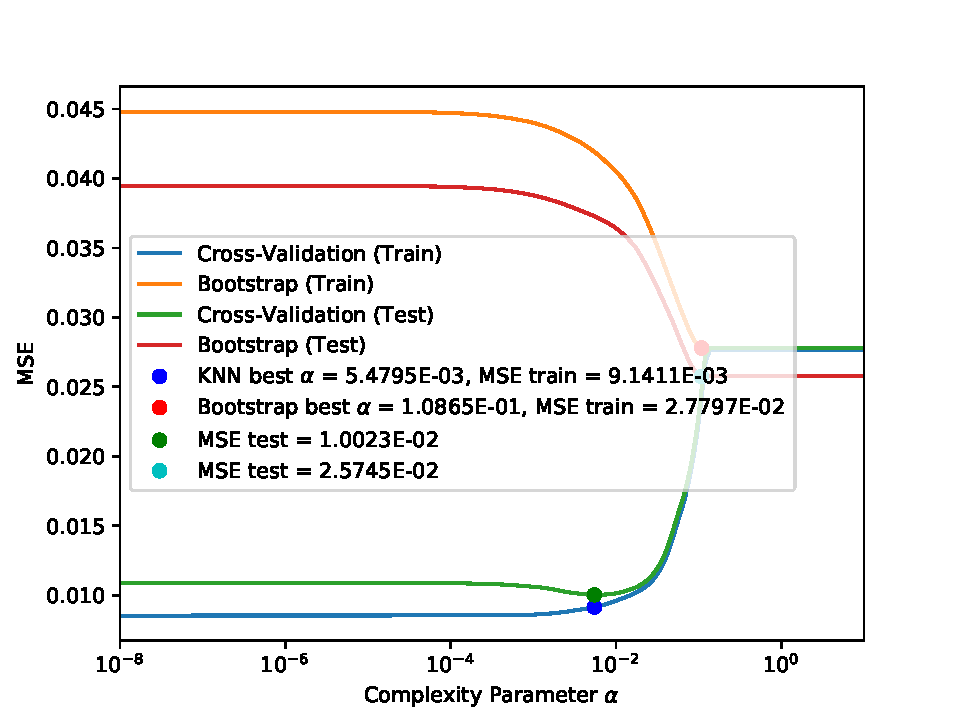
\includegraphics[width = 0.5\textwidth]{plot_1.pdf}
	\caption{A performance comparison between k-nearest-neighbors cross-validation and bootstrap, as a function of the complexity parameter $\alpha$.\label{fig_1}}
	\end{figure}
	
	\begin{figure}[H]
	\centering  
	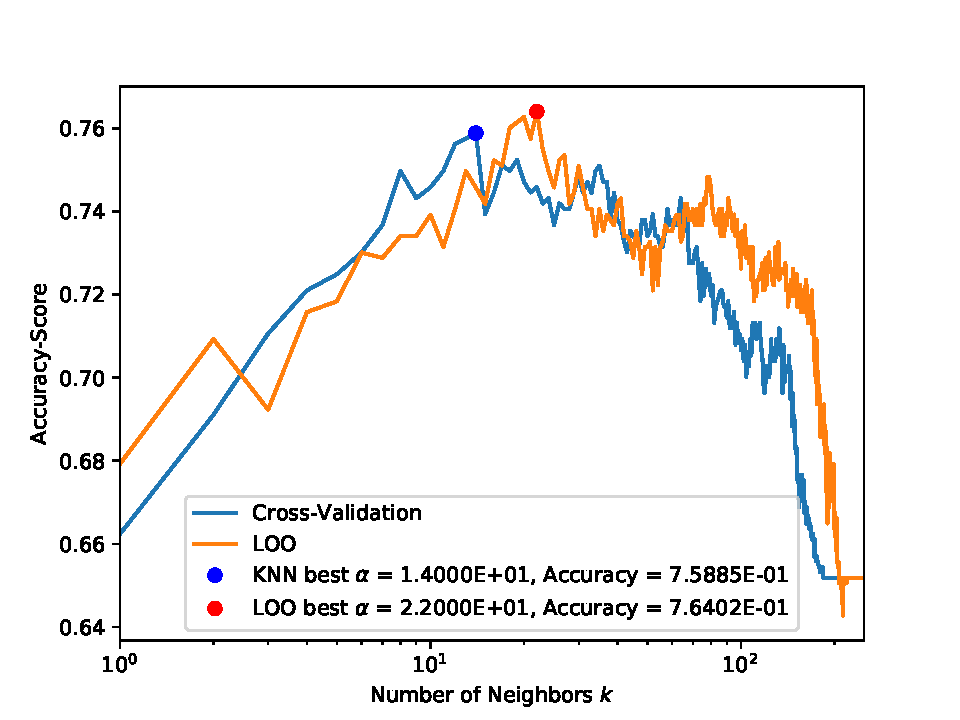
\includegraphics[width = 0.5\textwidth]{plot_2.pdf}
	\caption{A performance comparison between k-nearest-neighbors cross-validation and leave-one-out cross-validation, as a function of the number of neighbors $k$.\label{fig_2}}
	\end{figure}
	
	\begin{figure}[H]
	\centering  
	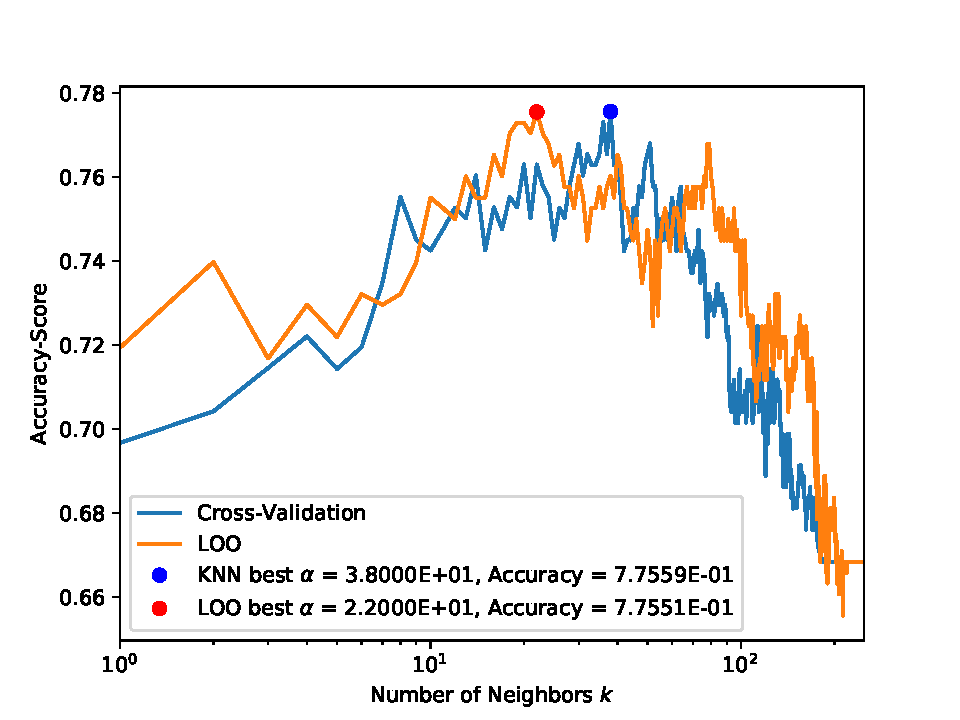
\includegraphics[width = 0.5\textwidth]{plot_3.pdf}
	\caption{A performance comparison between k-nearest-neighbors cross-validation and leave-one-out cross-validation, as a function of the number of neighbors $k$. For the filtered dataset.\label{fig_3}}
	\end{figure}
	
	\subsection{Source Code}
	
	\subsubsection{Snippets}
	
	\begin{figure}[H]
	\begin{lstlisting}[showstringspaces=false,language=Python,numbers=none]
	from sklearn.preprocessing import PolynomialFeatures
	from sklearn.model_selection import train_test_split
	from sklearn.model_selection import cross_validate
	from sklearn.preprocessing import StandardScaler
	from sklearn.preprocessing import MinMaxScaler
	import numpy as np
	
	with open("ozone_496obs_25vars.txt", "r") as infile:
	    data = infile.readlines()[1:]
	
	X,Y = [],[]
	
	for line in data:
	    line = line.split()
	    X.append(line[:-1])
	    Y.append(line[-1].strip())
	
	X = np.array(X).astype(np.float64)
	Y = np.array(Y).astype(np.float64)[:,np.newaxis]
	
	X_train, X_test, Y_train, Y_test = train_test_split(X, Y, test_size = 0.5)
	
	scaler = StandardScaler()
	X_train = scaler.fit_transform(X_train)
	X_test = scaler.transform(X_test)
	
	scaler = MinMaxScaler()
	Y_train = scaler.fit_transform(Y_train)
	Y_test = scaler.transform(Y_test)
	
	poly = PolynomialFeatures(1)
	X_test = poly.fit_transform(X_test)
	X_train = poly.fit_transform(X_train)
	\end{lstlisting}
	\caption{A preprocessing script for the \textit{forced vital capacity} dataset.\label{code_0}}
	\end{figure}
	
	\onecolumngrid	
	
	\subsubsection{Complete Source Code}
	
	The \texttt{python} scripts used to get these results is available on \texttt{github}:
	
	\begin{table}[H]
	\center
	\begin{tabular}{l c}
	\textbf{Problem 1} \ & \url{https://github.com/GabrielSCabrera/MachineLearning/blob/master/STK-IN4300/Oblig2/problem1.py} \\
	\textbf{Problem 2} \ & \url{https://github.com/GabrielSCabrera/MachineLearning/blob/master/STK-IN4300/Oblig2/problem2.py} 
	\end{tabular}
	\end{table}
	
	\subsection*{References}
	
	\bibliographystyle{ieeetr}
	\bibliography{bib}
	


	
\end{document}